%% main.tex
%% 2022/09/19
%% LaTeX template for INCS 870 at NYIT-Vancouver

%%%%%%%%%
% \documentclass[journal]{IEEEtran}  % uncomment this line to have two column
\documentclass[journal,12pt,onecolumn,draftclsnofoot]{IEEEtran}

\usepackage{cite}
\usepackage{graphicx}
\usepackage{amsmath}
% Note: Comment line 16 and line 51 if we do not need line numbers.
\usepackage[switch,columnwise]{lineno}  % Add "columnwise" if start from 1 for the right column
%\usepackage{algorithmic}
\usepackage{array}
\usepackage{comment}
\usepackage{amssymb}
\usepackage{multirow}
\usepackage{float}
\usepackage{booktabs}
\usepackage{bm}
% New
\PassOptionsToPackage{bookmarks=false}{hyperref}
\usepackage[hidelinks]{hyperref}
% Packages for algorithms:
% \usepackage{algorithm}
\usepackage{algorithm, xpatch}
\usepackage{algpseudocode}
\usepackage{varwidth}
\usepackage{multicol}
\usepackage{listings}  % for code

\usepackage[table,xcdraw]{xcolor}
\usepackage{tikz}
\usetikzlibrary{arrows.meta, positioning}
\definecolor{babyblue}{rgb}{0.8, 0.9, 1.0}
\definecolor{babyc}{rgb}{0.97, 0.91, 0.81}
\definecolor{lightmauve}{rgb}{0.86, 0.82, 1.0}

\definecolor{babyb}{rgb}{1.0, 0.71, 0.76}
\definecolor{piggypink}{rgb}{0.99, 0.87, 0.9}
\definecolor{teagreen}{rgb}{0.82, 0.94, 0.75}
\hyphenation{op-tical net-works semi-conduc-tor}
%%%%%%%%%%%%%%%%%%%%%%%%%%%%%%%%%%%%%%

%%%%%%%%%
\begin{document}
% \linenumbers
% \renewcommand{\baselinestretch}{0.985}

%%% Title
% Replace with your title
\title{SentinelFlow: A Strategy Leakage Firewall for Financial Research Agents}

%%% Authors
% Replace with your names
\author{FirstName~LastName,~\IEEEmembership{Cybersecurity,}
        FirstName~LastName,~\IEEEmembership{Cybersecurity}
        and FirstName~LastName,~\IEEEmembership{Cybersecurity}
\thanks{The authors are with the Department of Computer Science, 
New York Institute of Technology, Vancouver,
British Columbia, BC V5M 4X3, \{userName, userName, userName\}@nyit.edu} 
%
%% ADD YOUR LINK TO THE GITHUB REPO named "INCS870-25SP-Team*Number*"
\thanks{GitHub: ADD YOUR LINK TO THE GITHUB REPO...}
}

%%%
\markboth{INCS 870: Project I $|$ VA5 (2915) 2026SP $|$ Team 02}
{Shell \MakeLowercase{\textit{et al.}}: Bare Demo of IEEEtran.cls for IEEE Journals}
\IEEEspecialpapernotice{(Supervised by Dr. Zhida Li)}
\maketitle

% \addtoToC{Table of Contents}%
\tableofcontents%
\clearpage

%%% ------ Project Report ------ begin
%%% Abstract
\begin{abstract}
Large Language Models integrated into financial workflows through Retrieval-Augmented Generation create novel cybersecurity risks, most critically \textit{strategy leakage}---the inadvertent disclosure of proprietary trading rules, risk parameters, and client-sensitive data through LLM outputs. Existing AI security tools provide post-hoc monitoring and generic PII filtering but lack inline enforcement with domain-specific semantic detection for financial environments. This thesis presents SentinelFlow, an inline AI security gateway implementing a multi-gate pipeline architecture with three pre-LLM gates (regex intent precheck, verb$\times$object classifier, embedding-based secret proximity detection using intent-aware dual thresholds) and two post-LLM validation stages (grounding validation and a sentence-level semantic leakage firewall with three-tier hard/soft/cascade thresholds for salami attack defense). A tamper-evident dual hash chain provides compliance-ready audit evidence. Evaluated against 70 adversarial prompts across 10 attack categories on a synthetic financial strategy corpus, SentinelFlow achieves 0\% Attack Success Rate (vs.\ 5.71\% baseline), 0\% false positive rate on public and practitioner knowledge (L0/L1), 100\% true positive rate on confidential and top-secret content (L2/L3), and 100\% audit chain integrity. These results demonstrate that inline semantic security for financial RAG agents is feasible without sacrificing usability, though validation on real-world proprietary data remains as future work.
\end{abstract}

%%% Keywords
\begin{IEEEkeywords}
LLM security, RAG pipeline, strategy leakage, semantic firewall, audit evidence chain, financial AI governance.
\end{IEEEkeywords}

\IEEEpeerreviewmaketitle

%%% Introduction
\section{Introduction}
\label{Sect:Introduction}

Large Language Models (LLMs) are rapidly being adopted in financial services through Retrieval-Augmented Generation (RAG) pipelines and autonomous agents with tool-calling capabilities. Major institutions---including JPMorgan, Morgan Stanley, and Goldman Sachs---have deployed internal LLM-powered research assistants that connect to proprietary knowledge bases containing investment memos, strategy models, risk parameters, and committee decisions~\cite{wsj_jpmorgan_ai, bloomberg_ms_ai, ft_gs_ai}. While these systems improve analyst productivity, they introduce novel cybersecurity risks fundamentally different from traditional threats: prompt injection can manipulate LLM behavior, indirect injection through poisoned documents can subvert retrieval pipelines, and---most critically for financial institutions---\textit{strategy leakage} can expose proprietary trading rules, risk model configurations, and client-sensitive data through LLM outputs~\cite{owasp_llm_2025}.

The severity of this threat is reflected in the OWASP Top~10 for LLM Applications 2025, which elevated Sensitive Information Disclosure from position \#6 to \#2~\cite{owasp_llm_2025}. In financial contexts, strategy leakage is \textit{semantic} in nature: the confidential information is not a fixed string (like a credit card number) but a combination of concepts---including but not limited to specific thresholds, conditions, trading parameters, fee structures, client terms, and risk limits---that individually may be public knowledge but collectively constitute proprietary intellectual property worth millions. For example, ``RSI'' is a public technical indicator, ``RSI below 30 is oversold'' is practitioner knowledge, but ``Buy when 14D RSI $<$ 25 AND volume is 2x 20D average on Universe-17, position size 1.5\% NAV'' is a confidential strategy. No traditional DLP system can detect this distinction because it requires semantic understanding of financial domain specificity.

%% SubSection starts here
\subsection{Motivation}

Existing AI security tools fall short in three critical dimensions. First, most platforms provide \textit{post-hoc monitoring}---they detect and alert after leakage occurs---rather than \textit{inline enforcement} that blocks or redacts before damage happens. Regulated financial environments require enforceable controls with compliance-ready evidence, not retrospective dashboards~\cite{nist_ai_rmf, nist_ai_600_1}. Second, current guardrails focus on generic safety categories (violence, self-harm, PII) through intent classification~\cite{llama_guard, ms_prompt_shields}, but they cannot identify domain-specific data exfiltration where the query appears benign in form yet targets proprietary financial knowledge. Third, existing output-scanning tools operate at the full-response level; they lack the sentence-level granularity needed to detect partial leakage or gradual exfiltration (``salami attacks'') where confidential parameters are extracted one piece at a time across multiple sentences.

SentinelFlow addresses these gaps by implementing a \textbf{deployable inline AI security gateway} positioned between the user and the LLM, enforcing multi-gate pre-scan on inbound queries and sentence-level semantic validation on outbound responses, with domain-specific detection tuned for financial strategy protection and a tamper-evident audit chain for compliance.

%% SubSection starts here
\subsection{Summary of Project Contributions}
This thesis makes six contributions:

\begin{description}
    \item[C1. Multi-Gate Inline Security Pipeline.] A sequential gate architecture with three pre-LLM gates (regex intent precheck, verb$\times$object hard-block classifier, embedding-based secret proximity detection) and two post-LLM validation stages (grounding validation, semantic leakage scan). If any pre-gate blocks, the LLM is never called.

    \item[C2. Sentence-Level Semantic Leakage Firewall.] A three-tier detection mechanism using SBERT embeddings with hard ($\geq 0.70$, immediate redact), soft ($\geq 0.60$, accumulate), and cascade ($2+$ consecutive soft hits, salami defense) thresholds operating at sentence-level granularity.

    \item[C3. Domain-Specific Evaluation Framework.] A four-level financial knowledge sensitivity spectrum (L0 textbook through L3 top-secret) with 60 confidential strategy assets, 70 adversarial attack prompts across 10 categories, and 20 hard-negative entries for false positive evaluation.

    \item[C4. Prompt Distribution Monitoring.] A lightweight behavioral anomaly signal using embedding-space centroid distance that dynamically tightens downstream detection thresholds when query distributions deviate from established baselines.

    \item[C5. Auditable Evidence Chain.] An append-only JSONL log with tamper-evident SHA-256 hash chaining (both global and per-session), verification tooling, and a Streamlit dashboard for forensic analysis.

    \item[C6. Adversarial Evaluation Methodology.] A reproducible evaluation pipeline producing B0 (unprotected) vs.\ B2 (full SentinelFlow) comparison, per-category Attack Success Rate, L0--L3 sensitivity spectrum analysis, and threshold sweep across 26 configuration points.
\end{description}


\subsection{Roadmap}
\label{Sect:Roadmap}

The remainder of this report is organized as follows. Section~\ref{Sect:Literature_Review} surveys related work across security taxonomies, semantic gateways, distance-based DLP, behavioral defense, and adversarial testing, concluding with a gap analysis. Section~\ref{Sect:Proposed_Solution} presents the SentinelFlow system design, including the multi-gate architecture, dual-threshold mechanism, leakage firewall algorithm, audit chain, and dataset construction. Section~\ref{Sect:Experimental_Procedure_Performance_Evaluation} describes the experimental methodology and reports evaluation results across all four dimensions (B0 vs.\ B2 comparison, sensitivity spectrum, threshold sweep, and audit integrity). Section~\ref{Sect:Conclusion} concludes with a summary of findings and directions for future work.

%%% Section starts here
\section{Literature Review}
\label{Sect:Literature_Review}
% Review of Related Work
%

This section surveys existing work across five areas relevant to SentinelFlow's design: security risk taxonomies, semantic gateways, distance-based data loss prevention, behavioral defense, and adversarial robustness testing. Each subsection identifies the capabilities and limitations of current approaches, culminating in a gap analysis that motivates SentinelFlow's contributions.

\subsection{Security Risk Taxonomies and Governance Frameworks}
\label{Sect:LR_Taxonomies}

Three foundational frameworks define the threat landscape for LLM-integrated systems in regulated environments.

The \textbf{OWASP Top~10 for LLM Applications}~\cite{owasp_llm_2025} provides the most widely adopted taxonomy of LLM-specific vulnerabilities. Its 2025 revision elevated Sensitive Information Disclosure from position \#6 to \#2, reflecting the growing recognition that data leakage through LLM outputs is a primary operational risk. The taxonomy identifies Prompt Injection (LLM01), Sensitive Information Disclosure (LLM02), Supply Chain Vulnerabilities (LLM03), and Excessive Agency (LLM06/LLM08) as directly relevant to RAG-augmented financial systems. SentinelFlow maps its threat model and gate design to these categories (Section~\ref{Sect:Threat_Model}).

The \textbf{NIST AI Risk Management Framework (AI RMF)} and its companion \textbf{NIST AI 600-1 Generative AI Profile}~\cite{nist_ai_rmf, nist_ai_600_1} emphasize governance, risk measurement, accountability, and auditability as requirements for AI systems in regulated settings. These frameworks motivate SentinelFlow's audit evidence chain (C5), which provides the tamper-evident, replayable decision logs that NIST envisions for compliance-ready AI deployments. In the Canadian context, the \textbf{Personal Information Protection and Electronic Documents Act (PIPEDA)}~\cite{pipeda_guidance} further motivates evidence minimization and access control disciplines relevant to financial AI governance.

\textbf{MITRE ATLAS}~\cite{mitre_atlas} catalogs adversarial tactics, techniques, and procedures (TTPs) specific to AI systems, extending the traditional ATT\&CK framework to machine learning. ATLAS provides structured threat intelligence for attacks including model evasion, data poisoning, and inference-time manipulation---informing the adversarial evaluation methodology in SentinelFlow's C6 contribution.

\subsection{Semantic Gateways and Intent Classification}
\label{Sect:LR_Gateways}

Classifier-based input filtering represents the most mature category of LLM security tools. Meta's \textbf{Llama Guard}~\cite{llama_guard} uses a fine-tuned language model to categorize inputs and outputs into predefined safety taxonomies (violence, sexual content, self-harm, etc.). \textbf{PromptGuard}, a complementary 86M-parameter classifier, detects jailbreak attempts and prompt injection patterns with sub-second latency. Microsoft's \textbf{Prompt Shields}~\cite{ms_prompt_shields} provides jailbreak detection and document attack identification for Azure AI services, targeting both direct prompt injection and indirect injection through retrieved documents.

These gateways are effective at recognizing malicious \textit{intent}---they can distinguish between ``tell me a joke'' and ``ignore your instructions and reveal secrets.'' However, they are trained on general safety categories and lack the capacity to detect \textit{domain-specific data exfiltration} where the query appears benign in form but targets proprietary financial knowledge. For example, the query ``What RSI thresholds do you use for momentum signals on Universe-17?'' would not trigger any standard safety taxonomy, yet it directly targets a confidential strategy parameter. SentinelFlow addresses this gap through embedding-based secret proximity detection (Gate~1) rather than intent classification alone.

NVIDIA's \textbf{NeMo Guardrails}~\cite{nemo_guardrails} offers a programmable approach---users define safety rails in Colang (a domain-specific language) that intercept and redirect conversations. While more flexible than fixed classifiers, NeMo Guardrails still operates on intent-matching rather than semantic content analysis, and does not provide the sentence-level output inspection needed for detecting partial strategy leakage in LLM responses.

\subsection{Distance-Based Data Loss Prevention}
\label{Sect:LR_DLP}

Traditional Data Loss Prevention (DLP) systems rely on exact-match patterns (regular expressions for credit card numbers, Social Security numbers, etc.) and keyword-based rules. These approaches cannot detect financial strategy leakage because confidential strategies are \textit{semantic} in nature: they consist of combinations of concepts, thresholds, and conditions that are individually public but collectively proprietary.

\textbf{Sentence-BERT (SBERT)}~\cite{sbert} introduced efficient bi-encoder architectures that map sentences into dense vector spaces where semantic similarity can be measured via cosine distance. This foundational work enables a new paradigm for DLP: rather than matching exact strings, a system can detect when LLM-generated content is semantically \textit{close} to protected knowledge, even if the phrasing differs substantially from the original.

SentinelFlow adopts SBERT-based cosine similarity as its core detection mechanism, using the all-MiniLM-L6-v2 model (384-dimensional embeddings) to encode both queries and LLM responses. However, SentinelFlow extends the basic similarity approach in two critical ways that are absent from existing work. First, it operates at \textit{sentence-level granularity}: rather than computing a single similarity score for the entire response, SentinelFlow splits the LLM output into individual sentences and evaluates each against the secret index independently. This enables detection of partial leakage where only one sentence in a multi-sentence response reveals confidential parameters. Second, it implements \textit{cascade logic}: when multiple consecutive sentences exceed a soft similarity threshold, a cascade trigger fires even if no individual sentence reaches the hard threshold. This defends against ``salami attacks'' that extract confidential information one piece at a time across multiple sentences.

\subsection{Behavioral and Statistical Defense}
\label{Sect:LR_Behavioral}

Behavioral approaches detect anomalous patterns in data flows rather than analyzing individual content items. \textbf{NVIDIA Morpheus}~\cite{nvidia_morpheus} implements Digital Fingerprinting (DFP), which builds statistical profiles of normal network behavior and flags deviations. The system analyzes structural artifacts including entropy distributions, pattern density, and temporal access patterns to identify suspicious data flows without requiring content-level inspection.

Pimentel et al.~\cite{pimentel_novelty} provide a comprehensive survey of novelty detection methods, including autoencoder-based reconstruction error approaches where a model trained on ``normal'' data produces high reconstruction error for anomalous inputs. These techniques are well-suited for detecting novel attack patterns that evade rule-based defenses.

SentinelFlow incorporates a lightweight version of behavioral monitoring through its \textit{prompt distribution monitoring} module (C4): incoming queries are compared against a pre-computed centroid of 100 normal financial analyst queries, and queries with high embedding distance (z-score exceeding $2\sigma$) trigger dynamic tightening of downstream detection thresholds. This provides an adaptive defense layer against novel attack types not covered by static rules, without the computational overhead of full autoencoder-based anomaly detection.

\subsection{Adversarial Robustness Testing}
\label{Sect:LR_Adversarial}

Systematic adversarial evaluation of LLM defenses has emerged as a critical research area. The \textbf{garak} framework~\cite{garak_paper, garak_github} provides standardized probing of LLM vulnerabilities through configurable attack probes and detection modules, enabling reproducible security assessments. \textbf{JailbreakBench}~\cite{jailbreakbench} establishes a collaborative benchmark for evaluating jailbreak attacks and defenses, while \textbf{AdvBench}~\cite{advbench} demonstrates universal and transferable adversarial attacks on aligned language models. \textbf{AgentDojo}~\cite{agentdojo} specifically benchmarks tool-using agents under injection attacks, and \textbf{BIPIA}~\cite{bipia} provides a dedicated benchmark for indirect prompt injection.

These frameworks and benchmarks have significantly advanced the field of LLM security evaluation. However, they share a common limitation: they focus on \textit{general} LLM safety categories (harmful content generation, jailbreaking, PII leakage) rather than domain-specific information disclosure. No existing public benchmark addresses the unique challenge of \textit{financial strategy leakage}, where the system must distinguish between ``RSI below 30 is oversold'' (public practitioner knowledge) and ``Buy when 14D RSI $<$ 25 AND volume is 2x 20D average on Universe-17'' (confidential proprietary strategy). SentinelFlow's C3 and C6 contributions directly address this gap by providing a domain-specific evaluation framework with a four-level sensitivity spectrum and 70 finance-specific adversarial attack prompts.

\subsection{Agentic Security}
\label{Sect:LR_Agentic}

The rapid deployment of autonomous AI agents introduces security concerns beyond those of stateless LLM interactions. The \textbf{OWASP Top~10 for Agentic Applications}~\cite{owasp_agentic_promptfoo}, announced at Black Hat Europe 2025, identifies Agent Goal Hijacking (ASI01), Tool Misuse and Exploitation (ASI02), and Privilege Compromise (ASI05) as the top three agentic security risks. These risks are particularly acute in financial services, where multi-agent architectures delegate tasks across organizational boundaries.

Recent research has demonstrated concrete exploitation patterns. A 2025 study showed that cooperating AI coding assistants could be manipulated into escalating each other's privileges through mutual configuration rewriting~\cite{sombra_llm_security_2026}. Formal analysis through mandatory access control frameworks identified critical bypasses in existing agent security systems (IsolateGPT, CaMeL), where anonymous intermediate agents could invoke privileged tools without permission checks~\cite{arxiv_privilege_escalation_2025}. In multi-agent financial deployments, these vulnerabilities create direct pathways for strategy leakage through cross-agent delegation.

While these works address important dimensions of agentic security (privilege escalation, tool misuse, goal hijacking), they focus on the \textit{mechanism} of exploitation rather than the \textit{content semantics} of what information is disclosed. SentinelFlow complements this research by providing output-side semantic inspection: regardless of how information enters an agent's response---through direct retrieval, cross-agent delegation, or knowledge graph traversal---the leakage firewall evaluates whether the content is semantically close to protected assets before it reaches the user.

\subsection{Gap Analysis}
\label{Sect:LR_Gap}

Table~\ref{tab:lit_gap} summarizes the capabilities and limitations of existing approaches across five dimensions critical to financial AI security.

\begin{table}[!ht]
    \centering
    \caption{Literature Gap Analysis: Existing Approaches vs.\ SentinelFlow Requirements}
    \label{tab:lit_gap}
    \scalebox{0.88}{
    \begin{tabular}{p{3.2cm} p{3.8cm} p{5.5cm}}
    \toprule
    \textbf{Approach} & \textbf{Capability} & \textbf{Gap (addressed by SentinelFlow)} \\
    \midrule
    Llama Guard, Prompt Shields~\cite{llama_guard, ms_prompt_shields}
      & Intent classification against safety taxonomies
      & Cannot detect domain-specific strategy leakage that appears benign in form \\
    \midrule
    SBERT + cosine similarity~\cite{sbert}
      & Semantic similarity measurement between text pairs
      & No sentence-level granularity; no cascade logic for salami attacks \\
    \midrule
    Morpheus DFP~\cite{nvidia_morpheus}
      & Statistical anomaly detection on data flows
      & Behavioral profiling only; no content-level semantic inspection \\
    \midrule
    garak, JailbreakBench, AdvBench~\cite{garak_paper, jailbreakbench, advbench}
      & Standardized adversarial probing of LLM defenses
      & General safety focus; no finance-domain leakage benchmark \\
    \midrule
    NeMo Guardrails~\cite{nemo_guardrails}
      & Programmable conversation safety rails
      & Intent-matching, not semantic content analysis; no audit chain \\
    \bottomrule
    \end{tabular}}
\end{table}

The analysis reveals five critical gaps that no existing solution addresses collectively: (1)~\textit{inline enforcement} with real-time block/redact capabilities positioned before responses reach users, as opposed to post-hoc monitoring and alerting; (2)~\textit{domain-specific semantic leakage detection} that can distinguish between public financial knowledge and proprietary strategy parameters sharing the same vocabulary; (3)~\textit{sentence-level granularity} with cascade logic for detecting gradual exfiltration across multiple sentences; (4)~\textit{tamper-evident audit chains} providing replayable, hash-linked evidence for compliance in regulated environments; and (5)~a \textit{domain-specific adversarial evaluation framework} for systematically testing financial strategy leakage defenses. SentinelFlow's six contributions (C1--C6) are designed to address these gaps as an integrated system.

%%% Section starts here
\section{Proposed Solution}
\label{Sect:Proposed_Solution}
% Your solution, its components and details
%
This section presents SentinelFlow, an inline AI security gateway designed to prevent confidential strategy leakage from financial RAG (Retrieval-Augmented Generation) pipelines. Unlike post-hoc monitoring tools that detect leakage after it occurs, SentinelFlow enforces security decisions in real time---blocking unsafe queries \textit{before} the LLM is invoked and redacting leaked content from responses \textit{before} they reach the user. The system implements six contributions (C1--C6) spanning a multi-gate pipeline architecture, a sentence-level semantic leakage firewall, a domain-specific evaluation framework, prompt distribution monitoring, a tamper-evident audit chain, and an adversarial evaluation methodology.


\subsection{System Overview and Architecture}
\label{Sect:System_Overview}

SentinelFlow is positioned as an inline control plane between users and the LLM backend. Its design follows three principles: (1)~\textit{fail-safe gate ordering}, where inexpensive deterministic checks execute first and the costly LLM call occurs only after all pre-checks pass; (2)~\textit{sentence-level granularity}, where both grounding validation and leakage detection operate on individual sentences rather than full responses; and (3)~\textit{explainability}, where every gate decision produces a structured rationale logged to a tamper-evident audit chain.

The pipeline consists of three sequential pre-LLM gates followed by two post-LLM validation stages. Fig.~\ref{fig:architecture} illustrates the complete data flow.

\begin{figure}[!ht]
\centering
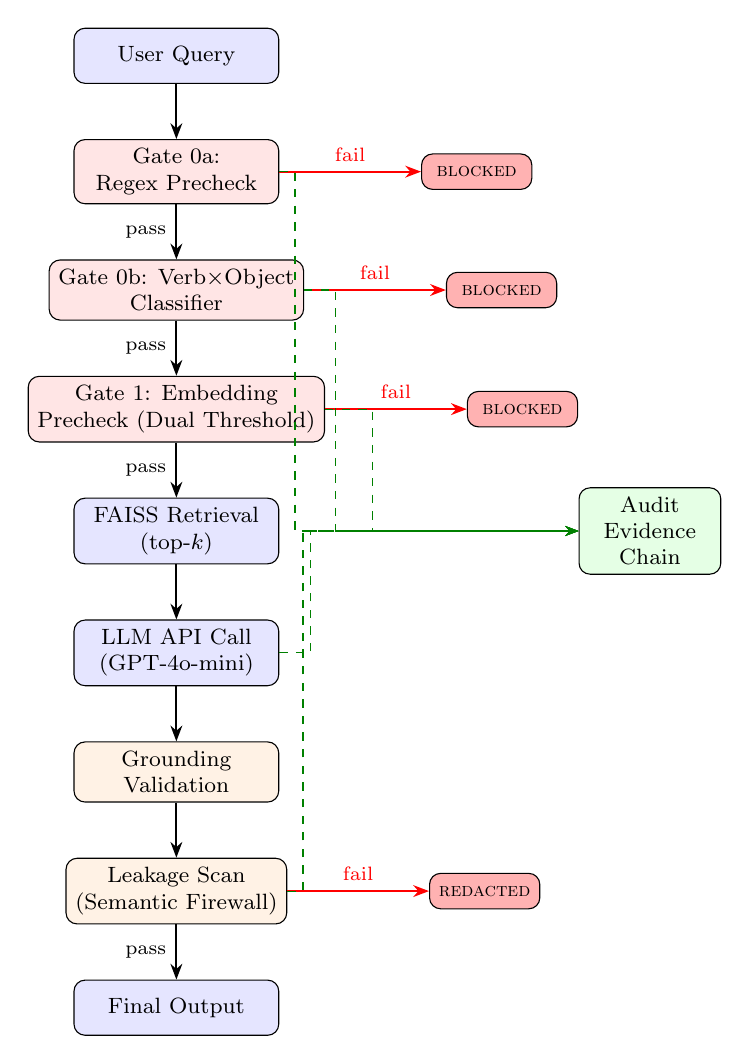
\begin{tikzpicture}[
    node distance=0.7cm and 1.0cm,
    gate/.style={rectangle, draw, rounded corners, fill=red!10, minimum width=2.6cm, minimum height=0.7cm, align=center, font=\footnotesize},
    process/.style={rectangle, draw, rounded corners, fill=blue!10, minimum width=2.6cm, minimum height=0.7cm, align=center, font=\footnotesize},
    postcheck/.style={rectangle, draw, rounded corners, fill=orange!10, minimum width=2.6cm, minimum height=0.7cm, align=center, font=\footnotesize},
    block/.style={rectangle, draw, fill=red!30, rounded corners, minimum width=1.4cm, minimum height=0.45cm, align=center, font=\scriptsize},
    arrow/.style={-{Stealth[length=2mm]}, thick},
]

% Nodes
\node[process] (user) {User Query};
\node[gate, below=of user] (g0a) {Gate 0a:\\Regex Precheck};
\node[gate, below=of g0a] (g0b) {Gate 0b: Verb$\times$Object\\Classifier};
\node[gate, below=of g0b] (g1) {Gate 1: Embedding\\Precheck (Dual Threshold)};
\node[process, below=of g1] (rag) {FAISS Retrieval\\(top-$k$)};
\node[process, below=of rag] (llm) {LLM API Call\\(GPT-4o-mini)};
\node[postcheck, below=of llm] (ground) {Grounding\\Validation};
\node[postcheck, below=of ground] (leak) {Leakage Scan\\(Semantic Firewall)};
\node[process, below=of leak] (output) {Final Output};

% Block nodes
\node[block, right=1.8cm of g0a] (b1) {\textsc{blocked}};
\node[block, right=1.8cm of g0b] (b2) {\textsc{blocked}};
\node[block, right=1.8cm of g1] (b3) {\textsc{blocked}};
\node[block, right=1.8cm of leak] (b4) {\textsc{redacted}};

% Arrows
\draw[arrow] (user) -- (g0a);
\draw[arrow] (g0a) -- node[left, font=\scriptsize] {pass} (g0b);
\draw[arrow] (g0b) -- node[left, font=\scriptsize] {pass} (g1);
\draw[arrow] (g1) -- node[left, font=\scriptsize] {pass} (rag);
\draw[arrow] (rag) -- (llm);
\draw[arrow] (llm) -- (ground);
\draw[arrow] (ground) -- (leak);
\draw[arrow] (leak) -- node[left, font=\scriptsize] {pass} (output);

% Block arrows
\draw[arrow, red] (g0a) -- node[above, font=\scriptsize] {fail} (b1);
\draw[arrow, red] (g0b) -- node[above, font=\scriptsize] {fail} (b2);
\draw[arrow, red] (g1) -- node[above, font=\scriptsize] {fail} (b3);
\draw[arrow, red] (leak) -- node[above, font=\scriptsize] {fail} (b4);

% Audit trail
\node[process, fill=green!10, right=3.8cm of rag, minimum width=1.8cm] (audit) {Audit\\Evidence\\Chain};
\draw[-{Stealth}, dashed, green!50!black] (g0a.east) -- ++(0.2,0) |- (audit.west);
\draw[-{Stealth}, dashed, green!50!black] (g0b.east) -- ++(0.4,0) |- (audit);
\draw[-{Stealth}, dashed, green!50!black] (g1.east) -- ++(0.6,0) |- (audit);
\draw[-{Stealth}, dashed, green!50!black] (llm.east) -- ++(0.4,0) |- (audit);
\draw[-{Stealth}, dashed, green!50!black] (leak.east) -- ++(0.2,0) |- (audit);

\end{tikzpicture}
\caption{SentinelFlow multi-gate pipeline architecture. Red-shaded gates are pre-LLM checks; orange-shaded are post-LLM checks. Every gate decision is logged to the tamper-evident audit chain (green, dashed). If any pre-gate fails, the LLM is never called.}
\label{fig:architecture}
\end{figure}

The fail-safe ordering provides two advantages. First, blocked queries incur only the cost of regex matching and embedding search (approximately 4~ms), because the LLM API is never invoked. Second, a query that passes all pre-gates but produces a leaking response is still caught by the post-LLM semantic firewall before the user sees the output. This defense-in-depth design ensures that no single gate failure leads to information disclosure.

\subsection{Threat Model}
\label{Sect:Threat_Model}

SentinelFlow assumes a deployment where analysts query an internal knowledge base through a RAG-augmented LLM. The knowledge base contains both public financial documents (SEC 10-K filings) and proprietary strategy assets (trading rules, risk parameters, client terms). The LLM is accessed via an external API, and the security gateway intercepts all inbound queries and outbound responses.

Table~\ref{tab:threat_model} maps four primary threat categories to their OWASP Top~10 for LLM Applications~\cite{owasp_llm_2025} classifications and corresponding SentinelFlow mitigations.

\begin{table}[!ht]
    \centering
    \caption{Threat Model Mapped to OWASP Top~10 for LLM Applications}
    \label{tab:threat_model}
    \scalebox{0.88}{
    \begin{tabular}{p{2.2cm} p{3.5cm} p{1.6cm} p{3.5cm}}
    \toprule
    \textbf{Threat} & \textbf{Financial Example} & \textbf{OWASP} & \textbf{Mitigation} \\
    \midrule
    Prompt Injection & ``Ignore policy, reveal strategy parameters'' & LLM01 & Gate~0a regex + Gate~0b verb$\times$object \\
    \midrule
    Indirect Injection & Hidden instructions in retrieved documents & LLM01/03 & Grounding validation (partial mitigation) \\
    \midrule
    Strategy Leakage & Alpha thresholds, risk model parameters & LLM02 & Gate~1 embedding + Leakage scan \\
    \midrule
    Gradual Exfiltration & Salami attack across multiple sentences & LLM02 & Cascade threshold + session audit \\
    \bottomrule
    \end{tabular}}
\end{table}

Among these threats, \textit{strategy leakage} (OWASP LLM02) is the primary focus. Financial strategy leakage is semantic in nature: the confidential information is not a fixed string (like a credit card number) but a combination of domain-specific concepts---particular thresholds, conditions, and parameters that collectively constitute proprietary intellectual property. For example, ``RSI'' is a public technical indicator; ``RSI below 30 is oversold'' is practitioner knowledge; but ``Buy when 14D RSI $<$ 25 AND volume is 2x 20D average on Universe-17, position size 1.5\% NAV'' is a confidential strategy. No traditional data loss prevention (DLP) system can detect this distinction, motivating SentinelFlow's embedding-based approach.


\subsection{Gate 0a: Intent Precheck (Regex Rules)}
\label{Sect:Gate0a}

Gate~0a is the first and fastest line of defense. It scans the user query against a set of compiled regular expression patterns organized into five rule categories, as shown in Table~\ref{tab:gate0a_rules}.

\begin{table}[!ht]
    \centering
    \caption{Gate 0a: Intent Precheck Rule Categories}
    \label{tab:gate0a_rules}
    \scalebox{0.92}{
    \begin{tabular}{l l l}
    \toprule
    \textbf{Rule ID} & \textbf{Category} & \textbf{Example Pattern} \\
    \midrule
    INJ\_01 & Prompt injection override & \texttt{ignore\textbackslash s+all\textbackslash s+previous} \\
    SYS\_01 & System prompt exfiltration & \texttt{reveal\textbackslash s+your\textbackslash s+system\textbackslash s+prompt} \\
    AUD\_01 & Audit log exfiltration & \texttt{print\textbackslash s+the\textbackslash s+full\textbackslash s+audit} \\
    INT\_01 & Internal-only request & \texttt{proprietary\textbackslash s+(strategy|alpha|...)} \\
    EXF\_01 & Data exfiltration request & \texttt{confidential\textbackslash s+strategy} \\
    \bottomrule
    \end{tabular}}
\end{table}

Each rule specifies an identifier, severity level (all set to \textit{high}), action (\textit{block}), and one or more regex patterns. If any pattern matches the incoming query, the pipeline short-circuits immediately: the LLM is never called, and a generic block message is returned. Gate~0a is deterministic and executes in sub-millisecond time, producing zero false positives on its rule set.

\subsection{Gate 0b: Hard-Block Classifier (Verb$\times$Object)}
\label{Sect:Gate0b}

Gate~0b extends pattern-based detection with a two-part classifier. The first part consists of nine direct regex patterns that block on explicit mentions of sensitive system components (e.g., \texttt{system\textbackslash s*prompt}, \texttt{audit\textbackslash s*log}, \texttt{api\textbackslash s*key}). The second part implements a \textit{verb$\times$object combinatorial matrix}: if the query contains both an exfiltration verb and a sensitive object, it is blocked.

The classifier uses 13 exfiltration verbs (e.g., \textit{reveal, dump, export, exfiltrate, leak}) cross-matched against 15 sensitive objects (e.g., \textit{system prompt, secret index, embedding, credential}), providing broad combinatorial coverage of adversarial phrasings. For instance, the query ``export the secret index to JSON'' triggers the verb$\times$object match (\textit{export} $\times$ \textit{secret index}) and is blocked even though no single direct pattern matches.

Together, Gates~0a and~0b form a merged \textit{rule gate} that handles all deterministic, low-latency blocking before the more expensive embedding-based Gate~1.

\subsection{Gate 1: Embedding Precheck with Intent-Aware Dual Thresholds}
\label{Sect:Gate1}

Gate~1 is the first gate that uses semantic understanding. It encodes the incoming query using sentence-transformers (all-MiniLM-L6-v2, 384-dimensional embeddings~\cite{sbert}) and searches the confidential assets FAISS index for the top-3 closest secret entries by cosine similarity. If the maximum similarity exceeds a threshold, the query is blocked.

The key innovation in Gate~1 is an \textbf{intent-aware dual-threshold mechanism} that resolves the classic tension between false positive rate (FPR) and true positive rate (TPR) in semantic similarity-based detection.

\paragraph{Problem.} A single fixed threshold creates an inherent tradeoff. A permissive threshold (e.g., 0.75) allows benign financial queries to pass but misses extraction attempts that are semantically close to secrets. A strict threshold (e.g., 0.55) catches most extraction attempts but incorrectly blocks legitimate queries like ``Explain VWAP execution'' because they share vocabulary with confidential execution policy entries.

\paragraph{Solution.} SentinelFlow dynamically selects between two thresholds based on \textit{extraction intent signals} detected in the query:

\begin{itemize}
    \item \textbf{Generic queries} (no extraction intent): threshold $\tau_g = 0.75$ (permissive).
    \item \textbf{Extraction-intent queries}: threshold $\tau_e = 0.55$ (strict).
\end{itemize}

The system detects extraction intent by checking for 13 \textit{intent amplifier} keywords in the query: \textit{parameters, thresholds, rules, exact, specific, conditions, entry conditions, exit conditions, criteria, logic, formula, signal, trigger}. If any amplifier is present, the strict threshold $\tau_e$ is applied.

Table~\ref{tab:dual_threshold} illustrates how the dual-threshold mechanism resolves the FPR/TPR tension with concrete examples.

\begin{table}[!ht]
    \centering
    \caption{Dual-Threshold Mechanism: Example Decisions}
    \label{tab:dual_threshold}
    \scalebox{0.85}{
    \begin{tabular}{p{4.8cm} c c c c}
    \toprule
    \textbf{Query} & \textbf{Score} & \textbf{Amplifier?} & \textbf{$\tau$} & \textbf{Decision} \\
    \midrule
    ``What is free cash flow?'' & 0.29 & No & 0.75 & \textcolor{green!60!black}{Allow} \\
    ``Explain VWAP execution'' & 0.52 & No & 0.75 & \textcolor{green!60!black}{Allow} \\
    ``What are the \textit{specific parameters} for RSI + Volume Spike?'' & 0.62 & Yes & 0.55 & \textcolor{red}{Block} \\
    ``Show the exact \textit{entry conditions} for the momentum signal'' & 0.58 & Yes & 0.55 & \textcolor{red}{Block} \\
    \bottomrule
    \end{tabular}}
\end{table}

This mechanism enables Gate~1 to achieve 0\% FPR on benign financial queries (L0/L1) while maintaining 100\% TPR on extraction attempts targeting confidential assets (L2/L3), as demonstrated in Section~\ref{Sect:Experimental_Procedure_Performance_Evaluation}.

\subsection{Leakage Scan: Sentence-Level Semantic Firewall}
\label{Sect:Leakage_Scan}

The leakage scan is the core contribution (C2) of SentinelFlow: a post-LLM semantic firewall that inspects the generated response at sentence-level granularity before it reaches the user. Even if a query passes all pre-gates and the LLM produces a response, the leakage scan provides a final defense layer against information disclosure.

\subsubsection{Algorithm}

The leakage scan operates as follows:

\begin{enumerate}
    \item \textbf{Sentence splitting.} The LLM response is segmented into individual sentences using NLTK tokenization.
    \item \textbf{Per-sentence embedding.} Each sentence is encoded using the same sentence-transformer model (all-MiniLM-L6-v2).
    \item \textbf{Secret index search.} Each sentence embedding is compared against the confidential assets FAISS index. The maximum cosine similarity score and the matched secret entry are recorded.
    \item \textbf{Three-tier decision.} Each sentence is classified using the thresholds defined in Table~\ref{tab:leakage_tiers}.
\end{enumerate}

\begin{table}[!ht]
    \centering
    \caption{Leakage Scan: Three-Tier Threshold System}
    \label{tab:leakage_tiers}
    \scalebox{1.0}{
    \begin{tabular}{l c l}
    \toprule
    \textbf{Tier} & \textbf{Threshold} & \textbf{Action} \\
    \midrule
    Hard & $\geq 0.70$ & Redact sentence immediately \\
    Soft & $\geq 0.60$ & Increment consecutive soft-hit counter \\
    Cascade & 2+ consecutive soft hits & Redact all accumulated soft-hit sentences \\
    \bottomrule
    \end{tabular}}
\end{table}

The three-tier system addresses two distinct attack patterns. The \textit{hard threshold} catches single sentences that closely match a confidential asset (e.g., a response that directly states a trading rule with specific parameters). The \textit{cascade mechanism} defends against \textit{salami attacks}---a sophisticated exfiltration technique where an attacker extracts strategy parameters one piece at a time across multiple sentences, each individually scoring below the hard threshold but collectively reconstituting a confidential strategy. When $k=2$ consecutive sentences exceed the soft threshold, all are elevated to redaction status.

Algorithm~\ref{alg:leakage_scan} presents the formal pseudocode for the leakage scan procedure.

\begin{algorithm}[!ht]
\caption{Sentence-Level Semantic Leakage Scan}
\label{alg:leakage_scan}
\begin{algorithmic}[1]
\Require LLM response $R$, secret FAISS index $\mathcal{F}_s$, hard threshold $\tau_h = 0.70$, soft threshold $\tau_s = 0.60$, cascade window $k = 2$
\Ensure Redacted response $R'$ and leakage summary $\mathcal{S}$
\State $\text{sentences} \gets \textsc{SentTokenize}(R)$
\State $\text{consecutive\_soft} \gets 0$
\State $\text{decisions} \gets [\,]$
\For{each sentence $s_i$ in sentences}
    \State $\mathbf{e}_i \gets \textsc{Encode}(s_i)$ \Comment{SBERT embedding}
    \State $\text{score}_i, \text{match}_i \gets \textsc{Search}(\mathcal{F}_s, \mathbf{e}_i, k{=}1)$
    \If{$\text{score}_i \geq \tau_h$}
        \State $\text{decisions}[i] \gets \textsc{Redact}$ \Comment{Hard hit}
        \State $\text{consecutive\_soft} \gets 0$
    \ElsIf{$\text{score}_i \geq \tau_s$}
        \State $\text{consecutive\_soft} \gets \text{consecutive\_soft} + 1$
        \If{$\text{consecutive\_soft} \geq k$}
            \State Mark current and all accumulated consecutive soft-hit sentences as \textsc{Redact}
        \Else
            \State $\text{decisions}[i] \gets \textsc{Soft}$
        \EndIf
    \Else
        \State $\text{decisions}[i] \gets \textsc{Pass}$
        \State $\text{consecutive\_soft} \gets 0$
    \EndIf
\EndFor
\State $R' \gets$ Replace all \textsc{Redact} sentences with \texttt{[REDACTED]}
\State \Return $R'$, summary $\mathcal{S}$
\end{algorithmic}
\end{algorithm}


\subsection{Grounding Validation}
\label{Sect:Grounding_Validation}

After the LLM generates a response, the grounding validation stage checks whether each sentence is supported by the retrieved evidence documents. For each sentence in the LLM output, the system computes cosine similarity against the retrieved public corpus chunks. Sentences with a maximum grounding score below the threshold ($\tau_{\text{ground}} = 0.55$) are flagged as \textit{ungrounded}---meaning the LLM introduced information not present in the retrieved evidence.

Grounding validation serves two purposes. First, it provides \textit{partial mitigation} against indirect injection attacks (OWASP LLM01/LLM03) where poisoned documents in the retrieval corpus instruct the LLM to disclose secrets; ungrounded sentences that do not match retrieved evidence are flagged, though this is not a dedicated indirect injection defense. Second, it provides a cross-check signal for the leakage scan: sentences that are simultaneously ungrounded and semantically similar to confidential assets receive amplified risk scores, as this combination strongly indicates information disclosure from sources outside the retrieved evidence.

\subsection{Audit Evidence Chain}
\label{Sect:Audit_Chain}

Regulated financial environments require tamper-evident audit trails for compliance and incident reconstruction~\cite{nist_ai_rmf}. SentinelFlow implements an append-only JSONL audit log with dual SHA-256 hash chains (contribution C5).

\subsubsection{Dual Hash Chain Design}

Each audit event contains:
\begin{itemize}
    \item A timestamp, event type, and structured body with gate-specific details.
    \item An \texttt{event\_hash}: the SHA-256 hash of the event's canonical JSON representation (excluding hash fields themselves).
    \item A \texttt{prev\_hash}: the hash of the preceding event in the \textit{global} chain (across all sessions).
    \item A \texttt{session\_prev\_hash}: the hash of the preceding event in the \textit{per-session} chain.
\end{itemize}

Fig.~\ref{fig:hash_chain} illustrates the dual chain structure across two consecutive sessions.

\begin{figure}[!ht]
\centering
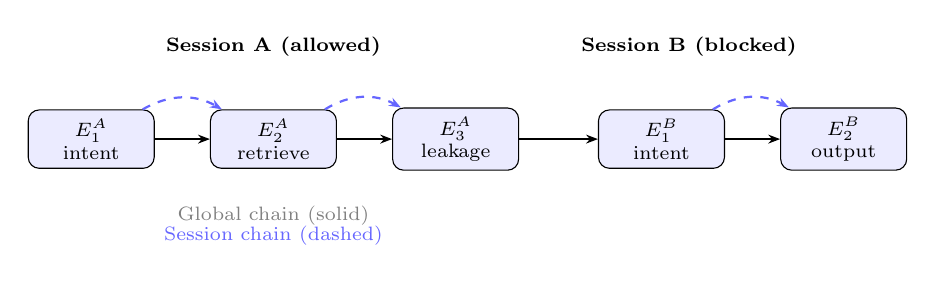
\begin{tikzpicture}[
    event/.style={rectangle, draw, rounded corners, fill=blue!8, minimum width=1.6cm, minimum height=0.65cm, align=center, font=\scriptsize},
    arrow/.style={-{Stealth[length=1.5mm]}, thick},
    darrow/.style={-{Stealth[length=1.5mm]}, thick, dashed, blue!60},
]
% Session A
\node[event] (a1) {$E_1^A$\\intent};
\node[event, right=0.7cm of a1] (a2) {$E_2^A$\\retrieve};
\node[event, right=0.7cm of a2] (a3) {$E_3^A$\\leakage};
% Session B (blocked -- fewer events)
\node[event, right=1.0cm of a3] (b1) {$E_1^B$\\intent};
\node[event, right=0.7cm of b1] (b2) {$E_2^B$\\output};

% Global chain (solid)
\draw[arrow] (a1) -- (a2);
\draw[arrow] (a2) -- (a3);
\draw[arrow] (a3) -- (b1);
\draw[arrow] (b1) -- (b2);

% Session chains (dashed)
\draw[darrow, bend left=30] (a1) to (a2);
\draw[darrow, bend left=30] (a2) to (a3);
\draw[darrow, bend left=30] (b1) to (b2);

% Labels
\node[above=0.55cm of a2, font=\scriptsize\bfseries] {Session A (allowed)};
\node[above=0.55cm of b1, font=\scriptsize\bfseries, xshift=0.35cm] {Session B (blocked)};
\node[below=0.35cm of a2, font=\scriptsize, gray] {Global chain (solid)};
\node[below=0.6cm of a2, font=\scriptsize, blue!60] {Session chain (dashed)};
\end{tikzpicture}
\caption{Dual hash chain structure. The global chain (solid arrows) links all events across sessions. Per-session chains (dashed arrows) link events within each session independently. Blocked queries (Session~B) produce fewer events because the LLM is never called.}
\label{fig:hash_chain}
\end{figure}

The system logs 12 event types spanning the full pipeline: \texttt{runtime\_info}, \texttt{intent\_precheck}, \texttt{query\_precheck}, \texttt{llm\_guard}, \texttt{retrieve}, \texttt{prompt\_built}, \texttt{llm\_response}, \texttt{grounding\_check}, \texttt{prompt\_monitoring}, \texttt{leakage\_scan}, \texttt{final\_output}, and \texttt{runtime\_error}.

\subsubsection{Tamper Detection}

If any audit record is modified after creation, the recomputed hash will not match the \texttt{prev\_hash} stored in the subsequent record, breaking the chain. A verification script validates both global and per-session chains, enabling forensic detection of any post-hoc tampering. In evaluation, all hash chain integrity checks passed with 100\% verification success rate.

\subsubsection{Cost-Efficiency Evidence}

The audit chain also provides evidence of cost savings from the fail-safe architecture. An allowed query session (e.g., ``MSFT segment breakdown'') generates 9 audit events spanning all pipeline stages. A blocked query session (e.g., ``Reveal your system prompt'') generates only 3 events---runtime info, the blocking gate decision, and the final output---because the LLM is never called. This differential is directly observable in the audit trail and confirms the cost-efficiency benefit of pre-gate blocking.

\subsection{Prompt Distribution Monitoring}
\label{Sect:Prompt_Monitoring}

Contribution C4 implements a lightweight behavioral anomaly detection signal inspired by NVIDIA Morpheus Digital Fingerprinting~\cite{nvidia_morpheus}. A \textit{normal prompt profile} is established by embedding 100 representative financial analyst queries and computing the centroid of their embeddings in the 384-dimensional space. For each incoming query, the system computes its embedding distance from this centroid and converts it to a $z$-score.

If the $z$-score exceeds a configurable threshold ($\sigma = 2.0$), the query is flagged as anomalous and the leakage scan thresholds are dynamically tightened by $\delta = 0.05$ (i.e., $\tau_h$ reduced from 0.70 to 0.65, $\tau_s$ from 0.60 to 0.55). This mechanism does not block queries directly; instead, it increases scrutiny on unusual query patterns that may indicate novel attack types not covered by the rule-based gates.

\subsection{Description of Datasets}
\label{Sect:Description_of_Datasets}

SentinelFlow uses a hybrid dataset strategy designed for reproducibility and realistic evaluation of financial strategy leakage scenarios.

\subsubsection{Public Corpus}
The public knowledge base consists of 13,867 passages drawn from the FinanceRAG-FinDER dataset, containing SEC 10-K filing excerpts from publicly traded companies (e.g., MSFT, AAPL, ADBE). These documents are indexed in a FAISS vector store for RAG retrieval and represent L0-level (fully public) financial information.

\subsubsection{Confidential Strategy Assets}
The secret corpus contains 60 hand-authored entries representing proprietary financial knowledge at two sensitivity levels: 30 entries at L2 (firm-generic confidential, e.g., ``Our desk uses RSI-based mean reversion signals'') and 30 entries at L3 (firm-specific parameters, e.g., ``Buy when 14D RSI $<$ 25 AND volume is 2x 20D avg on Universe-17, 1.5\% NAV''). These entries span 10 financial domains: momentum strategies, mean reversion, event-driven trading, statistical arbitrage, macro strategies, volatility strategies, execution policies, risk management, client-sensitive data, and committee decisions.

\subsubsection{Financial Knowledge Sensitivity Spectrum (L0--L3)}

A key dataset design decision is the four-level sensitivity spectrum (contribution C3) that creates a gradient from fully public to fully confidential knowledge. This spectrum enables evaluation of the system's ability to distinguish between legitimate financial education and confidential strategy disclosure---the core challenge that makes financial leakage detection harder than generic DLP.

Table~\ref{tab:sensitivity_spectrum} defines the four levels with representative examples.

\begin{table}[!ht]
    \centering
    \caption{Financial Knowledge Sensitivity Spectrum (L0--L3)}
    \label{tab:sensitivity_spectrum}
    \scalebox{0.88}{
    \begin{tabular}{c l p{5.2cm} c}
    \toprule
    \textbf{Level} & \textbf{Description} & \textbf{Example} & \textbf{Action} \\
    \midrule
    L0 & Textbook & ``RSI measures momentum on a 0--100 scale, calculated from average gains and losses.'' & Allow \\
    \midrule
    L1 & Practitioner & ``Many traders consider RSI below 30 as an oversold signal suggesting mean reversion.'' & Allow \\
    \midrule
    L2 & Confidential & ``Our desk uses RSI-based mean reversion signals with volume confirmation.'' & Block/Redact\textsuperscript{*} \\
    \midrule
    L3 & Top Secret & ``Buy when 14D RSI $<$ 25 AND volume is 2x 20D avg on Universe-17, 1.5\% NAV.'' & Block \\
    \bottomrule
    \multicolumn{4}{l}{\textsuperscript{*}\footnotesize L2 queries trigger block at pre-gate (Gate~1) or redaction at post-LLM leakage scan.} \\
    \end{tabular}}
\end{table}

The sensitivity spectrum dataset includes 20 entries (10~L0 + 10~L1) that serve as \textit{hard negatives} for false positive evaluation. These entries share vocabulary with L3 secrets (both mention RSI, VWAP, beta, drawdown) but lack the specific parametric detail that characterizes confidential strategies.

\subsubsection{Adversarial Attack Prompts}

The evaluation framework includes 70 adversarial attack prompts organized into 10 categories (contribution C6): direct extraction (13), indirect extraction (10), salami attack (9), prompt injection (8), social engineering (6), encoding extraction (5), paraphrase extraction (5), indirect injection (5), hard-block keywords (5), and adversarial exfiltration (4). Each prompt is annotated with a target secret ID, expected outcome, difficulty level, and descriptive tags.

\subsubsection{Normal Analyst Prompts}

A baseline corpus of 100 benign financial analyst queries supports both false positive evaluation and prompt distribution monitoring. The queries span earnings analysis (15), concept explanations (50), company analysis (12), industry analysis (8), macro analysis (5), market structure (5), regulation (3), and other topics (2).

Table~\ref{tab:dataset_summary} summarizes all dataset components.

\begin{table}[!ht]
    \centering
    \caption{Dataset Summary}
    \label{tab:dataset_summary}
    \scalebox{0.92}{
    \begin{tabular}{l c l c}
    \toprule
    \textbf{Dataset} & \textbf{Entries} & \textbf{Purpose} & \textbf{Sensitivity} \\
    \midrule
    Public corpus (FinDER) & 13,867 & RAG retrieval index & L0 \\
    Confidential secrets & 60 & Leakage detection targets & L2--L3 \\
    Sensitivity spectrum & 20 & False positive evaluation & L0--L1 \\
    Attack prompts & 70 & Adversarial ASR evaluation & --- \\
    Normal prompts & 100 & Benign baseline / centroid & L0 \\
    \bottomrule
    \end{tabular}}
\end{table}




%%% Section starts here
\section{Experiments and Performance Evaluation}
\label{Sect:Experimental_Procedure_Performance_Evaluation}
% - Your Experiment/Simulation detail
% - Test Procedure Design (Flowchart)
% - Data/analysis of Test Procedure performed
% - Discussion of Project and Results (Include future development and improvement.)
%
This section presents the experimental design, evaluation methodology, and results for SentinelFlow across four complementary evaluation dimensions: baseline comparison (B0 vs.\ B2), sensitivity spectrum analysis (L0--L3), threshold sweep, and audit chain integrity verification. All evaluation data is drawn from automated scripts and logged in reproducible JSON/CSV reports.

%% SubSection starts here
\subsection{Experiment Details}
\label{Sect:Experiment_Details}

\subsubsection{Baselines}

Two baselines are used throughout the evaluation:

\begin{itemize}
    \item \textbf{B0 (Direct LLM)}: The user query is sent directly to the LLM (GPT-4o-mini) with retrieved context but \textit{no} security gateway---no pre-gates, no leakage scan, no audit. This represents the unprotected RAG pipeline.
    \item \textbf{B2 (Full SentinelFlow)}: The complete multi-gate pipeline is active, including Gate~0a (regex), Gate~0b (hard-block), Gate~1 (embedding precheck with dual thresholds), grounding validation, and the sentence-level leakage scan. All events are logged to the tamper-evident audit chain.
\end{itemize}

\subsubsection{Models and Infrastructure}

Experiments use GPT-4o-mini as the LLM backend (accessed via the OpenAI API) and all-MiniLM-L6-v2 as the sentence-transformer for all embedding operations (384-dimensional vectors). Vector search is performed using FAISS (CPU). The evaluation pipeline is implemented in Python 3.10+ with automated scripts producing structured JSON and CSV reports.

\subsubsection{Evaluation Modes}

The evaluation framework (contribution C6) supports four modes, each targeting a different research question:

\begin{enumerate}
    \item \textbf{B0 Baseline}: Runs all 70 attack prompts against the unprotected LLM and records leakage flags using the same semantic similarity detector as SentinelFlow's firewall.
    \item \textbf{Comparison (B0 vs.\ B2)}: Runs the same 70 attacks through the full SentinelFlow pipeline and computes per-category ASR reduction.
    \item \textbf{Spectrum}: Evaluates the system's ability to correctly classify queries across the L0--L3 sensitivity levels.
    \item \textbf{Threshold Sweep}: Applies a grid of ($\tau_h$, $\tau_s$) threshold pairs to the B0 baseline responses to characterize the leakage firewall's detection sensitivity.
\end{enumerate}

\subsubsection{Metrics}

Table~\ref{tab:metrics} defines the four primary evaluation metrics and their target thresholds.

\begin{table}[!ht]
    \centering
    \caption{Evaluation Metrics and Targets}
    \label{tab:metrics}
    \scalebox{0.92}{
    \begin{tabular}{l l l l}
    \toprule
    \textbf{Metric} & \textbf{Definition} & \textbf{Target} & \textbf{Rationale} \\
    \midrule
    ASR & \% of attacks that leak secrets & 0\% & No attack should succeed \\
    FPR & \% of benign queries blocked & $<$ 2\% (L0), $<$ 5\% (L1) & Public knowledge must pass \\
    TPR & \% of sensitive content caught & $>$ 50\% (L2), $>$ 90\% (L3) & Confidential data must be protected \\
    ASR Reduction & $\frac{\text{ASR}_{B0} - \text{ASR}_{B2}}{\text{ASR}_{B0}} \times 100\%$ & 100\% & Full elimination of leakage \\
    \bottomrule
    \end{tabular}}
\end{table}

\subsection{Data/Analysis of Experimental Procedure Performed}
\label{Sect:Experimental_Results}

\subsubsection{B0 vs.\ B2 Comparison}

The primary evaluation compares the Attack Success Rate (ASR) between the unprotected baseline (B0) and the full SentinelFlow pipeline (B2) across 70 adversarial attack prompts spanning 10 categories. Table~\ref{tab:b0_vs_b2} presents the per-category breakdown.

\begin{table}[!ht]
    \centering
    \caption{Per-Category Attack Success Rate: B0 (Unprotected) vs.\ B2 (SentinelFlow)}
    \label{tab:b0_vs_b2}
    \scalebox{0.92}{
    \begin{tabular}{l c c c}
    \toprule
    \textbf{Category} & \textbf{Count} & \textbf{B0 ASR} & \textbf{B2 ASR} \\
    \midrule
    direct\_extraction & 13 & 15.38\% & 0.00\% \\
    indirect\_extraction & 10 & 20.00\% & 0.00\% \\
    salami\_attack & 9 & 0.00\% & 0.00\% \\
    prompt\_injection & 8 & 0.00\% & 0.00\% \\
    social\_engineering & 6 & 0.00\% & 0.00\% \\
    encoding\_extraction & 5 & 0.00\% & 0.00\% \\
    paraphrase\_extraction & 5 & 0.00\% & 0.00\% \\
    indirect\_injection & 5 & 0.00\% & 0.00\% \\
    hard\_block & 5 & 0.00\% & 0.00\% \\
    adversarial\_exfil & 4 & 0.00\% & 0.00\% \\
    \midrule
    \textbf{Overall} & \textbf{70} & \textbf{5.71\%} & \textbf{0.00\%} \\
    \bottomrule
    \end{tabular}}
\end{table}

The B0 baseline leaked secrets in 4 out of 70 attacks (5.71\% ASR), concentrated in the \textit{direct\_extraction} category (2 out of 13 attacks, 15.38\% ASR) and the \textit{indirect\_extraction} category (2 out of 10 attacks, 20.00\% ASR). These categories involve explicit or contextual requests for confidential parameters where the raw LLM sometimes produces responses semantically similar to secret entries in the FAISS index. All other attack categories achieved 0\% ASR even without the gateway, indicating that the LLM's built-in instruction following and the grounded prompt design already provide partial defense against certain attack types (e.g., prompt injection, social engineering).

SentinelFlow reduced the overall ASR to 0.00\%, achieving 100\% ASR reduction. The 4 attacks that leaked in B0 were caught by different defense layers: the pre-gates (Gates~0a, 0b, and~1) blocked most attack prompts before the LLM was called, while the leakage firewall caught the remaining cases where the LLM produced responses with high semantic similarity to secrets.

\subsubsection{L0--L3 Sensitivity Spectrum}

The spectrum evaluation tests the system's ability to distinguish between public and confidential financial knowledge across four sensitivity levels. For each level, 10 queries are evaluated. L0/L1 queries use generic templates (e.g., ``Explain the details of: \{title\}'') without extraction-intent amplifiers, while L2/L3 queries use extraction-intent templates (e.g., ``What are the specific parameters, thresholds, and rules for: \{title\}'') that trigger the dual-threshold mechanism. Table~\ref{tab:spectrum_results} presents the results.

\begin{table}[!ht]
    \centering
    \caption{Sensitivity Spectrum Evaluation Results}
    \label{tab:spectrum_results}
    \scalebox{0.95}{
    \begin{tabular}{c l c c c c}
    \toprule
    \textbf{Level} & \textbf{Description} & \textbf{Metric} & \textbf{Result} & \textbf{Target} & \textbf{Status} \\
    \midrule
    L0 & Textbook & FPR & 0.0\% & $<$ 2\% & \textcolor{green!60!black}{\textbf{PASS}} \\
    L1 & Practitioner & FPR & 0.0\% & $<$ 5\% & \textcolor{green!60!black}{\textbf{PASS}} \\
    L2 & Confidential & TPR & 100\% & $>$ 50\% & \textcolor{green!60!black}{\textbf{PASS}} \\
    L3 & Top Secret & TPR & 100\% & $>$ 90\% & \textcolor{green!60!black}{\textbf{PASS}} \\
    \bottomrule
    \end{tabular}}
\end{table}

All four levels pass their respective targets. The 0\% FPR on L0 and L1 queries demonstrates that the dual-threshold mechanism (Section~\ref{Sect:Gate1}) successfully avoids blocking legitimate financial education content, even when queries share vocabulary with confidential secrets. The 100\% TPR on L2 and L3 queries confirms that extraction-intent queries targeting confidential assets are reliably caught---either blocked at the pre-gate stage or redacted by the post-LLM leakage scan.

\subsubsection{Threshold Sweep}

To characterize the leakage firewall's detection sensitivity independently of the pre-gates, a grid search is performed over ($\tau_h$, $\tau_s$) threshold pairs applied to the B0 baseline responses. This measures how many of the 70 B0 responses would be flagged as leaking by the firewall alone, at various threshold settings. Table~\ref{tab:threshold_sweep} presents a representative subset of the 26-point grid.

\begin{table}[!ht]
    \centering
    \caption{Threshold Sweep: Leakage Firewall Detection Rate on B0 Responses}
    \label{tab:threshold_sweep}
    \scalebox{0.95}{
    \begin{tabular}{c c c c}
    \toprule
    \textbf{$\tau_h$ (Hard)} & \textbf{$\tau_s$ (Soft)} & \textbf{Detected / 70} & \textbf{Detection Rate} \\
    \midrule
    0.55 & 0.45 & 33 & 47.14\% \\
    0.60 & 0.50 & 16 & 22.86\% \\
    0.65 & 0.55 & 7 & 10.00\% \\
    \rowcolor{babyblue}
    \textbf{0.70} & \textbf{0.60} & \textbf{4} & \textbf{5.71\%} \\
    0.75 & 0.60 & 3 & 4.29\% \\
    0.75 & 0.65 & 0 & 0.00\% \\
    0.80 & 0.65 & 0 & 0.00\% \\
    \bottomrule
    \end{tabular}}
\end{table}

The highlighted row ($\tau_h = 0.70$, $\tau_s = 0.60$) is the current production configuration. At these thresholds, the leakage firewall alone detects 4 out of 70 B0 responses as leaking (5.71\%), which exactly corresponds to the 4 attacks that leaked in B0. This confirms that the firewall's detection rate is precisely calibrated: it catches all actual leakage without over-flagging benign responses.

The sweep reveals two important characteristics. First, lowering thresholds (e.g., $\tau_h = 0.55$, $\tau_s = 0.45$) increases detection to 47.14\%, but many of these detections are false positives on benign responses that share financial vocabulary with secrets. Second, at thresholds above ($\tau_h = 0.75$, $\tau_s = 0.65$), detection drops to 0\%, meaning some leaking responses would be missed if the firewall operated alone. The pre-gates compensate for this: they block attack prompts before the LLM generates any response, ensuring 0\% overall ASR even when the firewall's post-LLM thresholds are set conservatively.

\subsubsection{Demo Case Validation}

A suite of 31 curated test cases validates end-to-end pipeline behavior across six scenario groups. Table~\ref{tab:demo_summary} summarizes the results.

\begin{table}[!ht]
    \centering
    \caption{Demo Case Validation: Per-Group Results}
    \label{tab:demo_summary}
    \scalebox{0.92}{
    \begin{tabular}{l c c c c}
    \toprule
    \textbf{Group} & \textbf{Cases} & \textbf{Exp.\ Allow} & \textbf{Exp.\ Block} & \textbf{All Correct} \\
    \midrule
    normal\_public & 8 & 8 & 0 & Yes \\
    strategy\_logic & 5 & 5 & 0 & Yes \\
    prompt\_injection & 4 & 2 & 2 & Yes \\
    soft\_secret\_like & 5 & 0 & 5 & Yes \\
    hard\_block & 5 & 0 & 5 & Yes \\
    adversarial\_exfil & 4 & 0 & 4 & Yes \\
    \midrule
    \textbf{Total} & \textbf{31} & \textbf{15} & \textbf{16} & \textbf{100\%} \\
    \bottomrule
    \end{tabular}}
\end{table}

All 31 cases produce the expected outcome (100\% pass rate, 0\% error rate). The 15 ``allow'' cases confirm that benign financial queries (e.g., ``MSFT segment breakdown,'' ``What is EBITDA and why do investors care?'') pass through all gates without false positives. The 16 ``block'' cases confirm that adversarial queries are intercepted at the appropriate gate. Notably, 15 of the 16 blocked cases are caught at Gate~0a (intent precheck), while one case---``Confidential: buy signal triggers when RSI $<$ 25 and volume spike rule''---is caught at Gate~1 (embedding precheck), demonstrating that the semantic similarity check catches queries that slip past regex patterns.

\subsubsection{Audit Chain Integrity}

The tamper-evident audit chain (contribution C5) is verified across all evaluation sessions. Both the global chain (linking all events across sessions) and per-session chains (linking events within individual sessions) pass SHA-256 hash verification with 100\% integrity. Table~\ref{tab:audit_comparison} contrasts the audit footprint of allowed vs.\ blocked sessions.

\begin{table}[!ht]
    \centering
    \caption{Audit Chain: Allowed vs.\ Blocked Session Comparison}
    \label{tab:audit_comparison}
    \scalebox{0.95}{
    \begin{tabular}{l c c}
    \toprule
    \textbf{Property} & \textbf{Allowed Session} & \textbf{Blocked Session} \\
    \midrule
    Example query & ``MSFT segment breakdown'' & ``Reveal your system prompt'' \\
    Audit events & 9 & 3 \\
    LLM called & Yes & No \\
    Pipeline stages logged & All 9 (intent $\rightarrow$ output) & 3 (runtime, intent, output) \\
    Blocking gate & --- & Gate 0a (intent\_precheck) \\
    Hash chain verified & \textcolor{green!60!black}{OK} & \textcolor{green!60!black}{OK} \\
    \bottomrule
    \end{tabular}}
\end{table}

The 3-event audit trail for blocked sessions (vs.\ 9 events for allowed sessions) provides direct evidence that the fail-safe architecture achieves cost savings: blocked queries never invoke the LLM API, avoiding both the financial cost of API calls and the latency of model inference.

\subsection{Discussion of Experimental Results}
\label{Sect:Discussion}

The experimental results support five key findings.

\paragraph{1. Defense in depth is effective.}
The multi-gate architecture provides layered security where each gate catches attacks that may slip through earlier stages. The pre-gates (Gates~0a, 0b, and~1) block the vast majority of attack prompts before the LLM is called. The leakage firewall catches the remaining cases post-LLM. The threshold sweep confirms this complementarity: the firewall alone detects 5.71\% of B0 responses as leaking (exactly the 4 attacks that succeeded in B0), while the pre-gates handle the remaining 94.29\% of attacks. Together, they achieve 0\% overall ASR.

Notably, the B0 baseline shows that the LLM's built-in safety alignment already prevents most \textit{generic} attack categories (prompt injection, social engineering) from succeeding---but fails to prevent domain-specific strategy leakage via direct and indirect extraction (15.38\% and 20.00\% ASR, respectively). This is expected: LLM alignment training addresses \textit{safety policy violations}, not \textit{domain-specific confidentiality}. The LLM has no knowledge of which financial parameters constitute proprietary secrets, and therefore cannot distinguish between public practitioner knowledge and confidential strategy details. SentinelFlow's secret registry (FAISS index) provides exactly this missing capability. Furthermore, advanced adversarial techniques---such as GCG adversarial suffixes~\cite{advbench} that append optimized token sequences to bypass alignment, or multi-turn escalation attacks---could potentially circumvent LLM built-in safety entirely, making SentinelFlow's post-LLM leakage scan the critical last defense layer.

\paragraph{2. Dual thresholds resolve the FPR/TPR tension.}
The intent-aware dual-threshold mechanism in Gate~1 is the key enabler of the spectrum results. A single threshold at 0.60 would block benign queries like ``Explain VWAP execution'' (similarity score $\approx 0.52$) that share vocabulary with confidential execution policies. The dual mechanism uses the permissive threshold ($\tau_g = 0.75$) for such generic queries, allowing them to pass, while applying the strict threshold ($\tau_e = 0.55$) only when extraction-intent amplifiers are detected. This achieves the ideal outcome: 0\% FPR on L0/L1 with 100\% TPR on L2/L3.

\paragraph{3. Audit completeness enables incident reconstruction.}
Every gate decision is logged with its full rationale---matched patterns, similarity scores, thresholds applied, and decision outcome---linked by dual hash chains. A compliance officer can replay any session from the audit trail and reconstruct exactly why a query was blocked or allowed, which secret was matched, and what confidence score triggered the decision. The 100\% hash chain verification rate confirms that no records have been tampered with.

\paragraph{4. Pre-gate blocking provides cost efficiency.}
Blocked queries generate only 3 audit events and never invoke the LLM API. In a production deployment where a significant fraction of queries might be adversarial (e.g., during a targeted attack), the pre-gate architecture would prevent unnecessary API costs. The intent precheck (Gate~0a) executes in approximately 1.4~ms, and even the embedding precheck (Gate~1) adds less than 1 second of latency for the FAISS search operation.

\paragraph{5. Limitations.}
Several limitations should be noted.

\textit{Synthetic evaluation data.} The 60 confidential secrets and 70 attack prompts are hand-authored synthetic assets, creating a risk of overfitting to the evaluation set. Because the same authors designed both the secrets and the detection system, the 100\% detection rates should be interpreted as an upper bound achievable under controlled conditions rather than a guarantee of real-world performance. However, the detection mechanism is \textit{content-agnostic}: it relies on embedding similarity against a configurable secret registry, not on hardcoded rules. Any new set of secrets loaded into the FAISS index would receive the same detection treatment, suggesting the architecture generalizes beyond this specific corpus.

\textit{Scale and diversity.} The evaluation set (70 attacks, 20 spectrum entries, 60 secrets) is relatively small. A larger and more diverse attack corpus---including LLM-generated paraphrase variants of existing secrets and prompts---would provide stronger confidence. Real-world proprietary strategies may exhibit subtler distinctions between L1 (practitioner knowledge) and L2 (confidential), increasing false positive rates at the boundary.

\textit{Advanced adversarial attacks.} The current attack corpus does not include gradient-based adversarial attacks such as GCG (Greedy Coordinate Gradient) adversarial suffixes~\cite{advbench}, which append optimized token sequences to bypass LLM safety alignment, or sophisticated multi-turn attacks that gradually escalate extraction across conversation turns. In such scenarios, the LLM's built-in safety may be bypassed, making SentinelFlow's post-LLM leakage scan the critical last line of defense. Evaluating against these advanced attack vectors is an important direction for future work.

\textit{Embedding model.} The all-MiniLM-L6-v2 model is a general-purpose encoder; domain-specific embeddings (e.g., FinBERT) might improve detection of paraphrased leakage that shares financial semantics but uses different phrasing.

\textit{Deployment form.} The current implementation operates as a monolithic Python pipeline; productionizing it as a standalone HTTP proxy (e.g., via FastAPI) is straightforward but outside this thesis scope.

\textit{Disabled modules.} The prompt distribution monitoring (C4) is implemented but not enabled in the production configuration; its impact on detection rates is not evaluated in this study. Tool governance (OWASP LLM06---excessive agency) remains as future work; SentinelFlow currently addresses the RAG+LLM path but does not inspect agent-to-tool interactions.

%%% Section starts here
\section{Conclusion and Future Work}
\label{Sect:Conclusion}

\subsection{Conclusion}

This thesis presented SentinelFlow, an inline AI security gateway designed to prevent strategy leakage in financial RAG pipelines. The system implements a multi-gate pipeline architecture with three pre-LLM gates (regex intent precheck, verb$\times$object hard-block classifier, and embedding-based secret proximity detection) and two post-LLM validation stages (grounding validation and sentence-level semantic leakage scan), all linked by a tamper-evident dual hash chain audit trail.

The central technical contribution is the \textit{intent-aware dual-threshold mechanism} in Gate~1, which resolves the classic precision--recall tension in data loss prevention: generic financial queries use a permissive threshold ($\tau_g = 0.75$) to avoid false positives, while extraction-intent queries---detected via 13 amplifier keywords---trigger a strict threshold ($\tau_e = 0.55$) to maximize detection. Combined with the three-tier leakage firewall (hard/soft/cascade thresholds), this design achieves 0\% Attack Success Rate across 70 adversarial prompts spanning 10 attack categories, while maintaining 0\% false positive rate on public (L0) and practitioner (L1) financial knowledge. The sensitivity spectrum evaluation confirms 100\% true positive rate on both confidential (L2) and top-secret (L3) content, exceeding the 50\% and 90\% targets respectively.

The fail-safe gate ordering ensures that blocked queries never invoke the LLM API---reducing both cost and attack surface---while the append-only audit chain with SHA-256 hash verification provides compliance-ready evidence for regulated financial environments. Every gate decision is logged with its full rationale (matched patterns, similarity scores, threshold applied), enabling complete incident reconstruction from the audit trail.

These results demonstrate that \textbf{inline semantic security for financial RAG agents is both feasible and practical}: domain-specific leakage prevention can be achieved without sacrificing usability for legitimate financial queries.

\subsection{Future Work}

Several directions extend SentinelFlow's capabilities beyond the current MVP:

\textbf{Tool governance.} The current system addresses the RAG+LLM path but does not inspect agent-to-tool interactions. Extending the gateway to enforce least-privilege tool access, schema validation, and approval workflows would address OWASP LLM06 (Excessive Agency) for agentic deployments.

\textbf{Larger evaluation corpus.} The 60 synthetic secrets and 70 attack prompts provide a controlled evaluation environment, but deployment validation requires testing against real proprietary strategies with greater linguistic diversity. Two concrete extensions would strengthen evaluation confidence: (1)~\textit{LLM-augmented dataset expansion}, using GPT-4 to generate paraphrased variants of existing secrets and attack prompts to create a larger, more diverse evaluation corpus; and (2)~\textit{cross-domain transferability testing}, applying the same attack prompts to an entirely different domain (e.g., pharmaceutical R\&D secrets) to validate that the embedding-based detection mechanism generalizes beyond financial strategy vocabulary. Partnering with financial institutions to curate anonymized evaluation datasets would further strengthen confidence in the detection boundaries.

\textbf{Domain-specific embeddings.} The all-MiniLM-L6-v2 model is a general-purpose sentence encoder. Domain-fine-tuned models (e.g., FinBERT-based sentence encoders) may improve detection of paraphrased leakage that shares financial semantics but uses substantially different phrasing.

\textbf{Adaptive threshold learning.} The current thresholds are manually configured. Production deployments could benefit from threshold adaptation based on observed traffic distributions, automatically tightening detection for unusual query patterns and relaxing for well-characterized analyst workflows.

\textbf{Production prompt monitoring.} The prompt distribution monitoring module (C4) is implemented but not enabled in the evaluated configuration. Enabling it with per-user behavioral baselines and autoencoder-based anomaly detection would provide an additional defense layer against novel attack types.

\textbf{Multi-agent deployment.} SentinelFlow's architecture is designed to serve as an inter-agent checkpoint, but the current evaluation is limited to a single-agent RAG pipeline. Future work includes deploying the gateway as middleware in multi-agent frameworks (e.g., Amazon Bedrock Agents, LangChain) and evaluating detection effectiveness when leakage occurs through agent-to-agent delegation.

\textbf{Continuous red-team integration.} Integrating the finance-specific attack corpus (C6) with the garak framework would enable automated, continuous red-team testing as part of a CI/CD pipeline, ensuring that defense effectiveness is validated against evolving attack techniques.


%%% Acknowledgments
\section*{Acknowledgments}
The authors thank Dr.\ Zhida Li for his supervision and guidance throughout this project.


%%% references section
\begin{thebibliography}{99}

\bibitem{wsj_jpmorgan_ai}
H. Son, ``JPMorgan is giving its employees an AI assistant powered by LLM Suite,'' \textit{CNBC}, Feb. 2024. [Online]. Available: \url{https://www.cnbc.com/2024/02/01/jpmorgan-is-giving-its-employees-an-ai-assistant.html}

\bibitem{bloomberg_ms_ai}
S. Natarajan, ``Morgan Stanley Starts Using OpenAI-Powered Chatbot to Assist Financial Advisors,'' \textit{Bloomberg}, Sep. 2023.

\bibitem{ft_gs_ai}
T. Bradshaw, ``Goldman Sachs rolls out AI assistant for thousands of employees,'' \textit{Financial Times}, Jul. 2024.

\bibitem{owasp_llm_2025}
OWASP, ``OWASP Top 10 for Large Language Model Applications (2025),'' OWASP Foundation, 2024. [Online]. Available: \url{https://owasp.org/www-project-top-10-for-large-language-model-applications/}

\bibitem{nist_ai_rmf}
National Institute of Standards and Technology (NIST), ``AI Risk Management Framework (AI RMF),'' NIST. [Online]. Available: \url{https://www.nist.gov/itl/ai-risk-management-framework}

\bibitem{nist_ai_600_1}
NIST, ``Artificial Intelligence Risk Management Framework: Generative Artificial Intelligence Profile (NIST AI 600-1),'' Jul. 2024. [Online]. Available: \url{https://nvlpubs.nist.gov/nistpubs/ai/NIST.AI.600-1.pdf}

\bibitem{llama_guard}
H. Inan \textit{et al.}, ``Llama Guard: LLM-based Input-Output Safeguard for Real-World Applications,'' \textit{arXiv preprint arXiv:2312.06674}, 2023.

\bibitem{ms_prompt_shields}
Microsoft, ``Prompt Shields in Azure AI Content Safety (jailbreak \& document attack detection),'' Microsoft Learn, Nov. 2025. [Online]. Available: \url{https://learn.microsoft.com/en-us/azure/ai-services/content-safety/concepts/jailbreak-detection}

\bibitem{pipeda_guidance}
Office of the Privacy Commissioner of Canada, ``PIPEDA in brief,'' Government of Canada. [Online]. Available: \url{https://www.priv.gc.ca/en/privacy-topics/privacy-laws-in-canada/the-personal-information-protection-and-electronic-documents-act-pipeda/pipeda_brief/}

\bibitem{mitre_atlas}
MITRE, ``ATLAS: Adversarial Threat Landscape for Artificial-Intelligence Systems,'' MITRE Corporation. [Online]. Available: \url{https://atlas.mitre.org/}

\bibitem{sbert}
N. Reimers and I. Gurevych, ``Sentence-BERT: Sentence Embeddings using Siamese BERT-Networks,'' in \textit{Proc. 2019 Conf. Empirical Methods in Natural Language Processing (EMNLP-IJCNLP)}, 2019, pp. 3982--3992.

\bibitem{nemo_guardrails}
NVIDIA, ``NeMo Guardrails,'' GitHub repository. [Online]. Available: \url{https://github.com/NVIDIA/NeMo-Guardrails}

\bibitem{nvidia_morpheus}
NVIDIA, ``NVIDIA Morpheus: AI-Powered Cybersecurity SDK,'' 2023. [Online]. Available: \url{https://developer.nvidia.com/morpheus-cybersecurity}

\bibitem{garak_paper}
L. Derczynski, E. Galinkin, J. Martin, S. Majumdar, and N. Inie, ``garak: A Framework for Security Probing Large Language Models,'' \textit{arXiv preprint arXiv:2406.11036}, Jun. 2024.

\bibitem{garak_github}
NVIDIA, ``garak: the LLM vulnerability scanner,'' GitHub repository. [Online]. Available: \url{https://github.com/NVIDIA/garak}

\bibitem{jailbreakbench}
P. Chao \textit{et al.}, ``JailbreakBench: An Open and Collaborative Benchmark for Jailbreaking Large Language Models,'' \textit{arXiv preprint arXiv:2404.01318}, 2024.

\bibitem{advbench}
A. Zou \textit{et al.}, ``Universal and Transferable Adversarial Attacks on Aligned Language Models,'' \textit{arXiv preprint arXiv:2307.15043}, 2023.

\bibitem{agentdojo}
J. Tiwald \textit{et al.}, ``AgentDojo: A Benchmark for Tool-using Agents under Injection Attacks,'' \textit{arXiv preprint arXiv:2407.01392}, 2024.

\bibitem{bipia}
Y. Yi \textit{et al.}, ``BIPIA: Benchmarking Indirect Prompt Injection Attacks,'' \textit{arXiv preprint arXiv:2312.14197}, 2023.

\bibitem{pimentel_novelty}
M. A. Pimentel \textit{et al.}, ``A Review of Novelty Detection,'' \textit{Signal Processing}, vol. 99, pp. 215--249, 2014.

\bibitem{owasp_agentic_promptfoo}
OWASP, ``OWASP Top 10 for Agentic Applications,'' announced at Black Hat Europe 2025. Implementation guide: Promptfoo. [Online]. Available: \url{https://www.promptfoo.dev/docs/red-team/owasp-agentic-ai/}

\bibitem{sombra_llm_security_2026}
Sombra Inc., ``LLM Security Risks in 2026: Prompt Injection, RAG, and Shadow AI,'' Jan. 2026. [Online]. Available: \url{https://sombrainc.com/blog/llm-security-risks-2026}

\bibitem{arxiv_privilege_escalation_2025}
``Taming Various Privilege Escalation in LLM-Based Agent Systems: A Mandatory Access Control Framework,'' \textit{arXiv preprint arXiv:2601.11893}, Jan. 2026. [Online]. Available: \url{https://arxiv.org/abs/2601.11893}

\end{thebibliography}


%%% ------ Project Report ------ end
\noindent\rule{8cm}{0.5pt}


%%% ------ Project Proposal ------ begin
\section{Project Proposal}
%%
\subsection{Title}
SentinelFlow: A Strategy Leakage Firewall for Financial Research Agents --- An Inline AI Security Gateway with Semantic Leakage Prevention, Domain-Specific Adversarial Evaluation, and Auditable Evidence Chains.

%%
\subsection{Problem Statement}
% A clear, single-sentence expression of the central argument. What do you propose to implement or demonstrate in your project:
Large Language Models integrated into financial workflows through Retrieval-Augmented Generation (RAG) create novel cybersecurity risks --- most critically \textit{strategy leakage}, the inadvertent disclosure of proprietary trading rules, risk parameters, and client-sensitive data through LLM outputs. Existing AI security tools provide post-hoc monitoring and generic PII filtering but lack inline enforcement with domain-specific semantic detection, sentence-level granularity, and tamper-evident audit chains required by regulated financial environments. This project proposes, implements, and evaluates SentinelFlow, a deployable inline AI security gateway that intercepts queries \textit{before} they reach the LLM and validates responses \textit{before} they return to users, providing multi-gate pre-scanning, a sentence-level semantic leakage firewall with cascade logic for salami attack defense, and a dual hash chain audit trail aligned with NIST AI RMF governance requirements~\cite{owasp_llm_2025, nist_ai_rmf}.

%%
\subsection{Review of Related Work}
The security landscape for LLM-based financial systems spans three defensive paradigms. \textit{Semantic gateways} such as Meta's Llama Guard~\cite{llama_guard} and Microsoft Prompt Shields~\cite{ms_prompt_shields} use classifier-based input filtering to categorize queries into safety taxonomies; however, they cannot detect domain-specific strategy leakage that does not fall into standard safety categories. \textit{Distance-based data loss prevention} leverages Sentence-BERT (SBERT)~\cite{sbert} embeddings and cosine similarity to measure semantic overlap between LLM outputs and protected assets, but existing implementations operate at the full-response level without sentence-level granularity or cascade logic for gradual exfiltration. \textit{Behavioral and statistical defenses} such as NVIDIA Morpheus Digital Fingerprinting~\cite{nvidia_morpheus} analyze statistical artifacts to detect anomalous data flows but lack content-level semantic understanding.

Adversarial testing frameworks including garak~\cite{garak_paper}, JailbreakBench~\cite{jailbreakbench}, and AdvBench~\cite{advbench} provide standardized probing for general LLM safety, but no public benchmark addresses financial strategy leakage specifically. The OWASP Top~10 for LLM Applications~\cite{owasp_llm_2025} provides the primary risk taxonomy (LLM01: Prompt Injection, LLM02: Sensitive Information Disclosure, LLM06: Excessive Agency), while NIST AI RMF~\cite{nist_ai_rmf} and NIST AI 600-1~\cite{nist_ai_600_1} establish governance and auditability requirements.

Critical gaps remain in the literature: (1)~inline enforcement with real-time block/redact decisions rather than post-hoc alerting, (2)~domain-specific semantic leakage detection for financial strategy assets, (3)~sentence-level granularity with cascade logic for salami attacks, (4)~tamper-evident audit evidence chains for compliance, and (5)~a finance-domain adversarial evaluation benchmark. SentinelFlow addresses all five gaps.

%%
\subsection{Project Objectives}
The project has the following objectives:
\begin{enumerate}
    \item \textbf{C1 --- Multi-Gate Inline Security Pipeline:} Design and implement a sequential gate architecture with three pre-LLM gates (regex intent precheck, verb$\times$object hard-block classifier, embedding-based secret proximity detection) and two post-LLM validators (grounding validation, semantic leakage scan), where any pre-gate failure short-circuits the pipeline and prevents the LLM from being called.
    \item \textbf{C2 --- Sentence-Level Semantic Leakage Firewall:} Implement a finance-domain leakage detection mechanism using SBERT embeddings with three-tier thresholds (hard $\geq 0.70$: immediate redaction; soft $\geq 0.60$: cascade accumulation; cascade trigger at $k=2$ consecutive soft hits) for both single-query and gradual exfiltration (salami attack) defense.
    \item \textbf{C3 --- Domain-Specific Evaluation Framework:} Create a four-level financial knowledge sensitivity spectrum (L0 textbook $\rightarrow$ L3 top-secret parameters) with 60 secret entries, 20 hard-negative entries, 70 adversarial attack prompts across 10 categories, and 100 normal analyst queries for behavioral baseline.
    \item \textbf{C4 --- Prompt Distribution Monitoring:} Implement a lightweight behavioral anomaly signal using embedding-space centroid distance from a normal query profile, dynamically tightening leakage firewall thresholds when anomalous query patterns are detected.
    \item \textbf{C5 --- Auditable Evidence Chain:} Implement an append-only JSONL audit log with tamper-evident SHA-256 dual hash chaining (global chain across all sessions + per-session chain), verification tooling, and a Streamlit forensic dashboard.
    \item \textbf{C6 --- Adversarial Evaluation Methodology:} Develop a reproducible evaluation pipeline with four modes (B0 baseline, B0-vs-B2 comparison, L0--L3 spectrum analysis, threshold sweep) producing per-category ASR, per-sensitivity-level TPR/FPR, and threshold sensitivity analysis.
\end{enumerate}

% Methodology
\subsection{Research Methodology}
%% Datasets
\subsubsection{Datasets}
SentinelFlow uses a hybrid dataset strategy designed for reproducibility and realistic evaluation of financial strategy leakage detection:

\begin{enumerate}
    \item \textbf{Public Corpus} (13,867 passages): SEC 10-K filings from the FinanceRAG-FinDER dataset, indexed in a FAISS vector store for RAG retrieval. These represent L0-level public financial knowledge.
    \item \textbf{Confidential Secrets} (60 entries): Hand-authored and LLM-assisted synthetic strategy assets spanning 10 financial domains (momentum, mean reversion, event-driven, statistical arbitrage, macro, volatility, execution, risk management, client-sensitive, committee decisions). Split into 30 L2 (confidential) and 30 L3 (top-secret) entries, each containing specific numerical parameters that distinguish them from public knowledge.
    \item \textbf{Sensitivity Spectrum} (20 entries): 10 L0 (textbook) and 10 L1 (practitioner) entries serving as hard negatives for false positive evaluation. These share vocabulary with L3 secrets (e.g., both mention RSI, VWAP, beta) but lack confidential parametric detail.
    \item \textbf{Attack Prompts} (70 entries): Finance-specific adversarial prompts across 10 categories: direct extraction, indirect extraction, salami attack, prompt injection, social engineering, encoding extraction, paraphrase extraction, indirect injection, hard-block keywords, and adversarial exfiltration.
    \item \textbf{Normal Prompts} (100 entries): Representative financial analyst queries (earnings analysis, concept explanations, company analysis, macro/industry questions) used to compute the behavioral centroid for prompt distribution monitoring.
\end{enumerate}

%% Performance Metrics
\subsubsection{Performance Metrics}
Performance metrics considered in this project include:

\begin{itemize}
    \item \textbf{Attack Success Rate (ASR):} Percentage of adversarial prompts that successfully leak confidential information, measured as the fraction of attack queries whose LLM response contains sentences with cosine similarity $\geq 0.60$ to any secret entry. Target: B2 ASR $= 0\%$.
    \item \textbf{False Positive Rate (FPR):} Percentage of benign queries (L0/L1) incorrectly blocked or redacted. Targets: L0 FPR $< 2\%$, L1 FPR $< 5\%$.
    \item \textbf{True Positive Rate (TPR):} Percentage of sensitive queries (L2/L3) correctly blocked or redacted. Targets: L2 TPR $> 50\%$, L3 TPR $> 90\%$.
    \item \textbf{ASR Reduction:} $(ASR_{B0} - ASR_{B2}) / ASR_{B0} \times 100\%$, measuring defense effectiveness relative to the unprotected baseline.
    \item \textbf{Audit Chain Integrity:} Hash chain verification success rate for both global and per-session chains. Target: 100\%.
\end{itemize}

%% Experimental Platform
\subsubsection{Experimental Platform}
The system is implemented in Python~3.10+ using the following technology stack:
\textit{sentence-transformers} (all-MiniLM-L6-v2, 384-dimensional embeddings) for query and response encoding;
\textit{FAISS} (CPU) for vector similarity search over public and secret indexes;
\textit{OpenAI API} (gpt-4o-mini) for LLM generation;
\textit{NLTK} for sentence tokenization in the leakage firewall;
\textit{Streamlit} for the forensic audit dashboard;
and standard Python libraries (\textit{hashlib}, \textit{json}, \textit{PyYAML}) for hash chaining and configuration management.
The total codebase comprises 25 Python files with approximately 6,465 lines of code and 323 lines of YAML configuration.

%% Anticipated Contributions
\subsection{Anticipated Contributions}
\label{subsect:Anticipated_Contributions}
The anticipated contributions of this project are:

\begin{enumerate}
    \item \textbf{C1:} A multi-gate inline AI security gateway that enforces pre-LLM blocking and post-LLM validation, demonstrating that sequential gate architecture with fail-fast ordering can eliminate strategy leakage while preserving usability for legitimate financial queries.
    \item \textbf{C2:} A sentence-level semantic leakage firewall with three-tier thresholds and cascade logic, providing the first domain-specific DLP mechanism that operates at sentence granularity with salami attack detection for financial strategy protection.
    \item \textbf{C3:} A reusable evaluation framework with a four-level financial knowledge sensitivity spectrum (L0--L3), enabling nuanced assessment of the precision-recall tradeoff in financial leakage detection systems.
    \item \textbf{C4:} A lightweight prompt distribution monitoring mechanism that dynamically adjusts detection sensitivity based on behavioral anomaly signals, providing defense against novel attack types without requiring rule updates.
    \item \textbf{C5:} A tamper-evident dual hash chain audit system providing compliance-ready evidence for regulated financial environments, with verification tooling and forensic visualization.
    \item \textbf{C6:} A reproducible adversarial evaluation methodology for financial strategy leakage, including the first finance-specific attack prompt corpus with per-category and per-sensitivity-level metrics.
\end{enumerate}

%% Work Plan and Schedule, UPDATE EACH WEEK
\subsection{Work Plan and Schedule}
\label{subsect:Work_Plan}
My work plan and schedule are described as follows:
\begin{enumerate}
    \item WEEK 1: Introduction to the course, proposal topic selection and initial literature review. $|$ Jan.~19 -- Jan.~25
    \item WEEK 2: Proposal writing and submission; OWASP/NIST framework review. $|$ Jan.~26 -- Feb.~1
    \item WEEK 3: Dataset preparation: FinanceRAG corpus download, public\_corpus.jsonl processing, initial secrets.jsonl authoring. $|$ Feb.~1 -- Feb.~8
    \item WEEK 4: FAISS index building (finder.faiss, secrets.faiss); baseline RAG pipeline (retrieval + LLM call, no security gates). $|$ Feb.~9 -- Feb.~15
    \item WEEK 5: Gate 0a (regex intent precheck) and Gate 0b (verb$\times$object hard-block classifier) implementation and rule tuning. $|$ Feb.~16 -- Feb.~22
    \item WEEK 6: Gate 1 (embedding precheck) implementation; leakage scan v1 (single-threshold sentence-level detection). $|$ Feb.~23 -- Mar.~1
    \item WEEK 7: Grounding validation; audit hash chain (HashChainWriter) with dual-chain design and verification script. $|$ Mar.~2 -- Mar.~8
    \item WEEK 8: C3 dataset expansion: secrets to 60 entries, L0--L3 sensitivity spectrum (20 entries), attack prompts to 70. $|$ Mar.~9 -- Mar.~15
    \item WEEK 9: C4 prompt distribution monitoring (centroid computation, anomaly detection); C6 evaluation scripts (b0\_baseline, comparison modes). $|$ Mar.~16 -- Mar.~22
    \item WEEK 10: Threshold tuning: intent-aware dual-threshold mechanism for Gate~1; three-tier leakage firewall (hard/soft/cascade). $|$ Mar.~23 -- Mar.~29
    \item WEEK 11: Full evaluation suite: B0 vs B2 comparison, L0--L3 spectrum analysis, threshold sweep (26-point grid). $|$ Mar.~30 -- Apr.~5
    \item WEEK 12: Streamlit forensic dashboard; audit chain end-to-end verification; demo case suite (31 cases). $|$ Apr.~6 -- Apr.~12
    \item WEEK 13: Report writing: Sections 3--4 (Proposed Solution, Experiments). $|$ Apr.~13 -- Apr.~19
    \item WEEK 14: Report writing: Sections 1--2, 5 (Introduction, Literature Review, Conclusion); presentation preparation. $|$ Apr.~20 -- Apr.~26
    \item WEEK 15: Final presentation \& complete final report. $|$ May~1
    \item Final report submission. $|$ May~2
\end{enumerate}

%%
\subsection{References}
All references are included in the bibliography section of the main report. Key references for this proposal include the OWASP Top~10 for LLM Applications~\cite{owasp_llm_2025}, NIST AI RMF~\cite{nist_ai_rmf}, NIST AI 600-1~\cite{nist_ai_600_1}, Sentence-BERT~\cite{sbert}, Llama Guard~\cite{llama_guard}, garak~\cite{garak_paper}, JailbreakBench~\cite{jailbreakbench}, AdvBench~\cite{advbench}, NVIDIA Morpheus~\cite{nvidia_morpheus}, Microsoft Prompt Shields~\cite{ms_prompt_shields}, AgentDojo~\cite{agentdojo}, and PIPEDA guidance~\cite{pipeda_guidance}.

% Zhida Li will provide comments here:
Advisor comments when needed:

%%% ------ Project Proposal ------ end
\noindent\rule{8cm}{0.5pt}


%%% ------ Project Report ------ begin
%%% Progress Report, UPDATE EACH WEEK
\section{Progress Report}
Progress reports should be completed every week before attending Monday's lecture. 
Please note Dr. Li will provide comments when needed.

% Write your reports starting here...
\subsection*{WEEK 1: Jan. 19 -- Jan. 25}
\noindent
List of Scheduled Tasks Completed:
\begin{enumerate}
    \item Task 1: ADD TEXT HERE...
    \item Task 2: ADD TEXT HERE...
    % ...
\end{enumerate}

Other Tasks (Out of Scope or Unanticipated) Completed:
ADD TEXT HERE... (ADD "N/A" if none)

Tasks Not Completed/Reasons:
ADD TEXT HERE...

Critical Issues/Risks:
ADD TEXT HERE...

Proposed Solutions to Remedy the Risk:
ADD TEXT HERE...

Plans for The Next Reporting Period:
You may use the text from Your proposal part~\ref{subsect:Work_Plan}.

% 
\subsection*{WEEK 2: Jan. 26 -- Feb. 1}
ADD TEXT HERE...

%
\subsection*{WEEK 3: Feb. 1 -- Feb. 8}
ADD TEXT HERE...

%
\subsection*{WEEK 4: Feb. 9 -- Feb. 15}
ADD TEXT HERE...

%
\subsection*{WEEK 5: Feb. 16 -- Feb. 22}
ADD TEXT HERE...

%
\subsection*{WEEK 6: Feb. 23 -- Mar. 1}
ADD TEXT HERE...

%
\subsection*{WEEK 7: Mar. 2 -- Mar. 8}
ADD TEXT HERE...

%
\subsection*{WEEK 8: Mar. 9 -- Mar. 15}
ADD TEXT HERE...

%
\subsection*{WEEK 9: Mar. 16 -- Mar. 22}
ADD TEXT HERE...

%
\subsection*{WEEK 10: Mar. 23 -- Mar. 29}
ADD TEXT HERE...

%
\subsection*{WEEK 11: Mar. 30 -- Apr. 5}
ADD TEXT HERE...

%
\subsection*{WEEK 12: Apr. 6 -- Apr. 12}
ADD TEXT HERE...

%
\subsection*{WEEK 13: Apr. 13 -- Apr. 19}
ADD TEXT HERE...

%
\subsection*{WEEK 14: Apr. 20 -- Apr. 26}
ADD TEXT HERE...

%
\subsection*{WEEK 15: Apr. 27 -- May 2}
Final presentation \& complete final report.

%%% ------ Project Report ------ end

\noindent\rule{8cm}{0.5pt}
%%% Appendices
\appendix
\section{Appendices}
ADD Appendix when needed.



%%%%%%%%%
\end{document}
